\section{}
\textit{A machine of 100 kg mass is supported on springs of total stiffness 700 kN/m and has an unbalanced rotating element, which results in a disturbing force of 350 N, at the speed of 3000 rpm. Assuming a damping ratio of $\zeta = 0.2$:}
\begin{figure}[H]
    \centering
    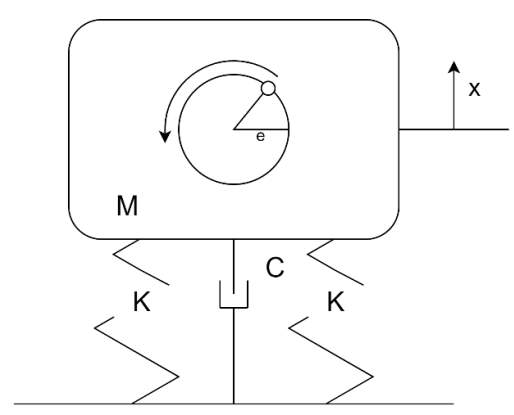
\includegraphics[width=0.5\linewidth]{Questions/Figures/Q4 Problem Diagram.png}
\end{figure}
\begin{enumerate}[label=(\alph*)]
    \item \textit{The amplitude of motion of the machine due to the unbalance.}
    \item \textit{The transmissibility and the transmitted force to the base.}
\end{enumerate}

\subsection*{Solution}
\subsection{}
This is a forced damped system with rotating imbalance. The amplitude of vibration is given from Eq. (4.11),
\begin{align*}
    \mathbb{X} &= \frac{F_o/k}{\sqrt{\left[1 - \left(\frac{\omega}{p} \right)^2 \right]^2 + \left[2 \zeta \frac{\omega}{p} \right]^2}}
\end{align*}
All parameters are known except $p$. The natural frequency is
\begin{align*}
    p &= \sqrt{\frac{k}{m}} = \sqrt{\frac{700 \times 10^3}{100}} \times \frac{60}{2\pi} = 798.95 \text{ RPM}
\end{align*}
then,
\begin{align*}
    \mathbb{X} &= \frac{350/(700\times 10^3)}{\sqrt{\left[1 - \left(\frac{3000}{798.95} \right)^2 \right]^2 + \left[2 \times 0.2 \times \frac{3000}{798.95} \right]^2}} \\
    &= \boxed{3.792 \times 10^{-5} \text{ m}}
\end{align*}

\subsection{}
